
\chapter{Cape of Good Hope - Postal History 
} 
\chapter{Cape - Stamps Perkins Bacon Issue 1853
} 
\begin{marginfigure}
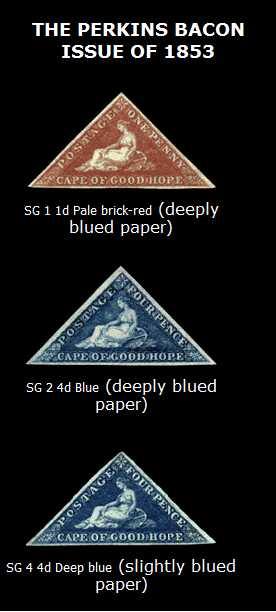
\includegraphics[width=1.0\textwidth]{../cape-of-good-hope/bacon.jpg}
\end{marginfigure}
  	 
The first issue of the triangular stamps of the Cape of Good Hope were engraved and printed by Messrs. Perkins, Bacon & Co.

The stamps were despatched to the Cape on the 11th May, 1853. They arrived a month later and the consignement was lodged at the Treasury Offices of the Cape. The Perkins Bacon issue was the first time that the Cape of Good Hope issued stamps.

The stamps were designed by Bell the Cape of Good Hope surveyor. The choice of the triangular shape is alleged to have been chosen so that the illiterate could distinguish the Cape of Good Hope stamps from those of other countries.

The stamps were advertized in the Cape Government Gazette of the 18th August 1853. In the same issue of the Cape Government Gazette 
the Postmaster General published, a long list of persons, holding retail licenses in the Cape of Good Hope Colony, with whom arrangements were made for the sale of postage stamps.

Thus the first stamps of the Cape of Good Hope were put on Sale on 1st September 1853.
The Design of the Cape Stamps

The design of the stamps as can be seen from the above illustrations represents a female figure of Hope sitting upon an anchor, which rests upon a rock. The background consists of fine engine-turned lines.
Paper Used in the Production of the Cape Stamps

The paper used for the printing of the Cape triangular stamps was especially manufactured to the meet the particular requirements of the triangular stamps of the Cape of Good Hope. This paper was exclusively used for all the printings.

The paper is white wove varying considerably in texture. The gum is a pale brown. the gum was applied after the printing was done.

A particular aspect of this issue was the 'blueing of the paper'. This was caused entirely by the type of inks used for the printing. This effect was notable in most issues printed by Perkins, Bacon & Co. at the time for Great Britain and its colonies.

This problem was later fixed during the printing of the Second Triangular Issue

\subsection{Watermark of the Cape Triangle Stamps
} 
The watermark used in the production of the Cape stamps was the familiar anchor in double outline. The watermark designs (technically known as 'bits') were arranged so that each stamp had one anchor standing upright, with the 'ring' underneath the apex of the triangle.

Most of the Cape triangular stamps are known with the watermark sideways. These stamps are the result of the paper being fed into the printing machine reversed, i.e. turned over so that the printing was done on the wrong side of the sheet.

 

       